\documentclass[glossy]{beamer}
\useoutertheme{wuerzburg}
\useinnertheme[realshadow,corners=2pt,padding=2pt]{chamfered}
\usecolortheme{shark}

\usepackage{listings}
\usepackage[utf8]{inputenc}

\usepackage{tikz}
\newcommand<>{\hover}[1]{\uncover#2{%
 \begin{tikzpicture}[remember picture,overlay]%
 \draw[fill,opacity=0.4] (current page.south west)
 rectangle (current page.north east);
 \node at (current page.center) {#1};
 \end{tikzpicture}}
}

\title{Concurso PAD - Área Arquitectura de Computadoras\\\line(1,0){320}}
% \author{\texorpdfstring{Author\newline\url{email@email.com}}{Author}}
%\author{Rafael Ignacio Zurita}
\institute{Rafael Ignacio Zurita \\ Departamento de Ingenieria de Computadoras \\ Clase de oposición}
%\date{\today}



\begin{document}




\begin{frame}
\maketitle
\end{frame}

\institute{Rafael Zurita - Departamento de Ingenieria de Computadoras - FAI - UNCOMA \\ 2018}

\begin{frame}
\frametitle{Programa Analítico}
	\begin{center}
\textbf{Jerarquía de Memoria}
	\end{center}
\begin{itemize}
\item Computador actual y renovación (que comprar)
\item Los programadores quisieron siempre ilimitada cantidad de memoria
\item tendencia de las ultimas decadas en el diseño tecnológico de CPU y memoria principal
\begin{itemize}
\item Las cpu se diseñaron con mejor performance, las memorias principales (DRAM) se diseñaron con el objetivo de ser mas densas y baratas, luego performance
\end{itemize}
\item Tecnología actual ya vista (UNIDAD II) flip-flops D para registros y memoria statica
\item Idea clave: tener los datos correctos, en el lugar preciso, en el momento adecuado
\begin{itemize}
\item Y que significa lo anterior: analogia del alumno y el examen (papel, lapiz, calculadora)
\end{itemize}

\item Principio de localidad
\item Jerarquía de memoria: ilimitada cantidad de la memoria más rápida al menor costo
\end{itemize}
\end{frame}


\begin{frame}
\frametitle{Jerarquía de Memoria}
\begin{center}
\textbf{Jerarquía de Memoria}
\end{center}

\begin{itemize}
\item Test
\end{itemize}

\begin{center}
\end{center}
\begin{center}
\begin{figure}
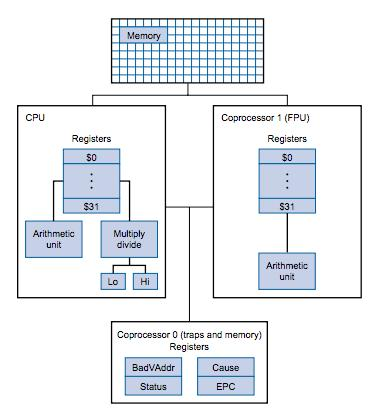
\includegraphics[scale=0.4]{organizacion-mips.jpg} 
\caption{Diagrama de Bloques de una computadoroa MIPS}
\label{Diagrama de Bloques de una computadoroa MIPS}
\end{figure}
\end{center}
\end{frame}









\begin{frame}
\frametitle{Jerarquía de memoria}
        \begin{center}
        \textbf{Cuando se quiere comprar una computadora nueva...}
        \end{center}
Si ya contamos con una PC CPU core i3 2.6Ghz, 8GB RAM, 512GB disco, \textbf{¿Qué computadora queremos adquirir?:}
\begin{tabular}{cl}

\begin{tabular}{c}
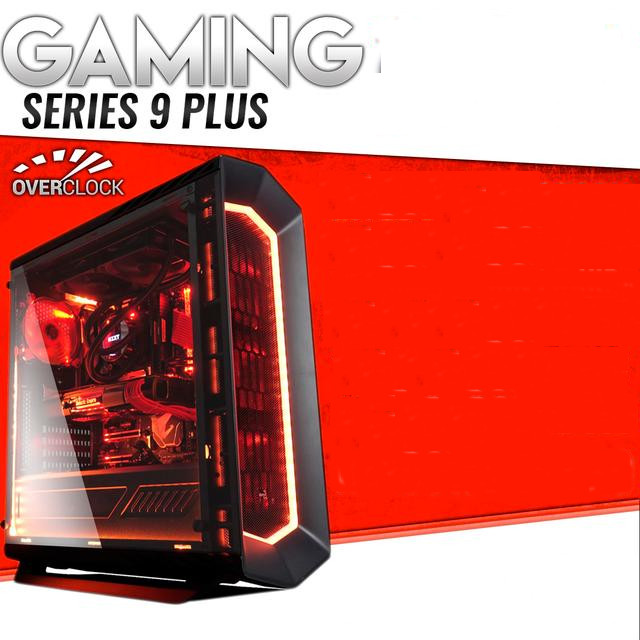
\includegraphics[height=6cm, width=4cm]{pc5.jpg} 

\end{tabular}
& \begin{tabular}{l}
\parbox{0.5\linewidth}{
        \textbf{Procesador}: ..................... \\
        \textbf{Memoria}: ..................... \\
        \textbf{Disco}: ..................... 
}
\end{tabular} \\

\end{tabular}
\end{frame}




\begin{frame}
\frametitle{Jerarquía de memoria}
        \begin{center}
        \textbf{Cuando se quiere comprar una computadora nueva...}
        \end{center}
Si ya contamos con una PC CPU core i3 2.6Ghz, 8GB RAM, 512GB disco, \textbf{¿Qué computadora queremos adquirir?:}
\begin{tabular}{cl}

\begin{tabular}{c}
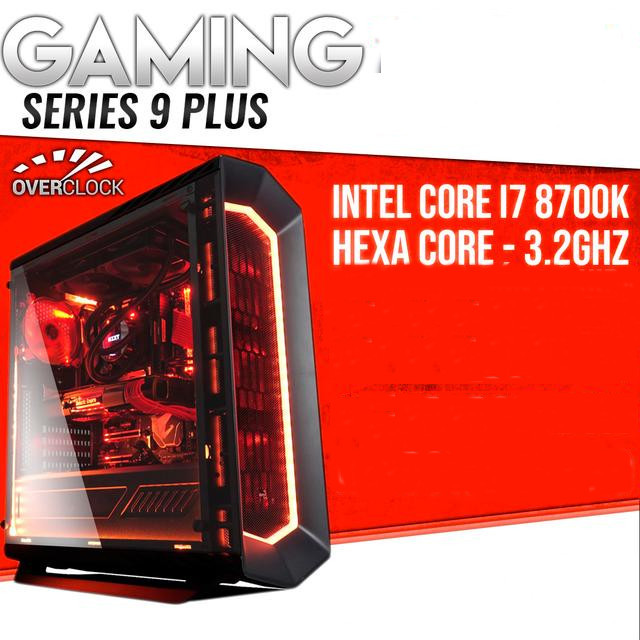
\includegraphics[height=6cm, width=4cm]{pc45.jpg} 

\end{tabular}
& \begin{tabular}{l}
\parbox{0.5\linewidth}{
        \textbf{Procesador}: más rápido, mas cores \\
        \textbf{Memoria}: ..................... \\
        \textbf{Disco}: ..................... 
}
\end{tabular} \\

\end{tabular}
\end{frame}



\begin{frame}
\frametitle{Jerarquía de memoria}
        \begin{center}
        \textbf{Cuando se quiere comprar una computadora nueva...}
        \end{center}
Si ya contamos con una PC CPU core i3 2.6Ghz, 8GB RAM, 512GB disco, \textbf{¿Qué computadora queremos adquirir?:}
\begin{tabular}{cl}

\begin{tabular}{c}
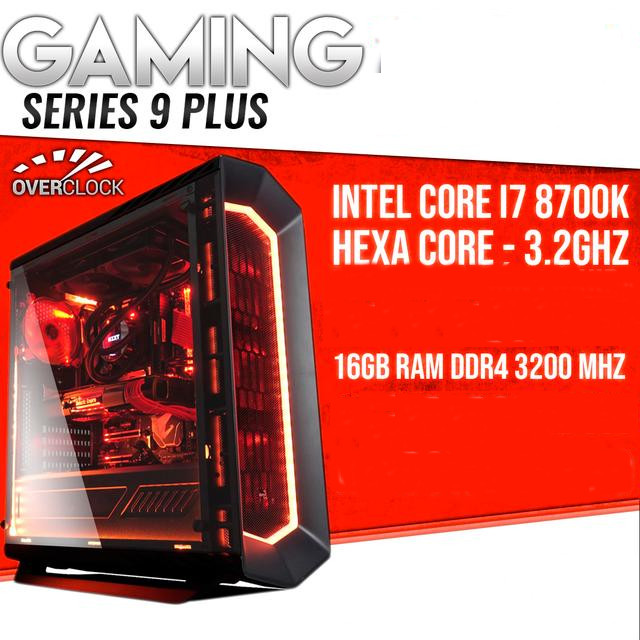
\includegraphics[height=6cm, width=4cm]{pc4.jpg} 

\end{tabular}
& \begin{tabular}{l}
\parbox{0.5\linewidth}{
        \textbf{Procesador}: más rápido, mas cores \\
        \textbf{Memoria}: más memoria \\
        \textbf{Disco}: ..................... 
}
\end{tabular} \\

\end{tabular}
\end{frame}



\begin{frame}
\frametitle{Jerarquía de memoria}
        \begin{center}
        \textbf{Cuando se quiere comprar una computadora nueva...}
        \end{center}
Si ya contamos con una PC CPU core i3 2.6Ghz, 8GB RAM, 512GB disco, \textbf{¿Qué computadora queremos adquirir?:}
\begin{tabular}{cl}

\begin{tabular}{c}
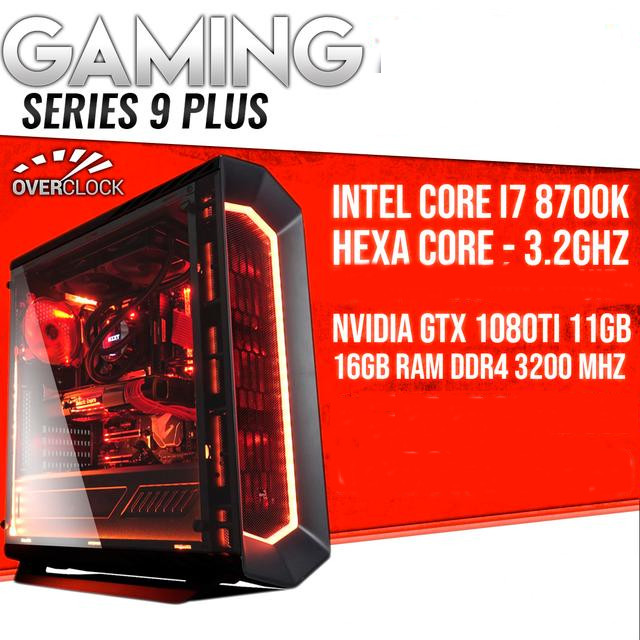
\includegraphics[height=6cm, width=4cm]{pc3.jpg} 

\end{tabular}
& \begin{tabular}{l}
\parbox{0.5\linewidth}{
        \textbf{Procesador}: más rápido, mas cores \\
        \textbf{Memoria}: más memoria \\
        \textbf{Disco}: ..................... 
}
\end{tabular} \\

\end{tabular}
\end{frame}






\begin{frame}
\frametitle{Jerarquía de memoria}
        \begin{center}
        \textbf{Cuando se quiere comprar una computadora nueva...}
        \end{center}
Si ya contamos con una PC CPU core i3 2.6Ghz, 8GB RAM, 512GB disco, \textbf{¿Qué computadora queremos adquirir?:}
\begin{tabular}{cl}

\begin{tabular}{c}
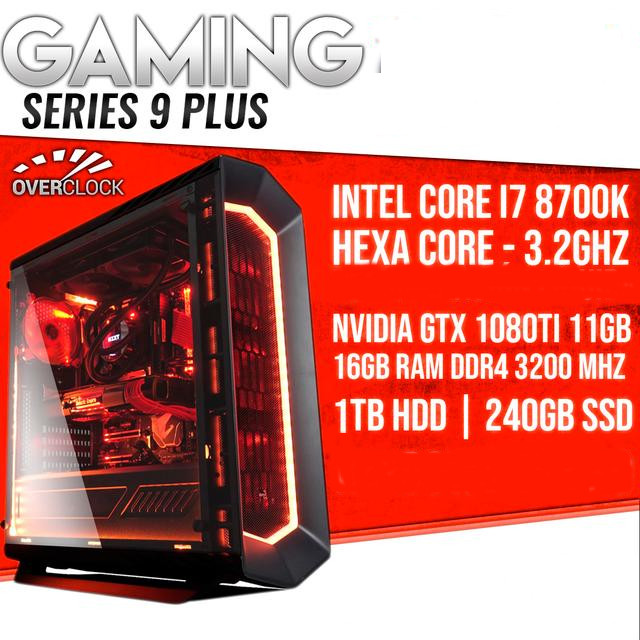
\includegraphics[height=6cm, width=4cm]{pc2.jpg} 

\end{tabular}
& \begin{tabular}{l}
\parbox{0.5\linewidth}{
        \textbf{Procesador}: más rápido, mas cores \\
        \textbf{Memoria}: más memoria \\
        \textbf{Disco}: más disco 
}
\end{tabular} \\

\end{tabular}
\end{frame}






\begin{frame}
\frametitle{Jerarquía de memoria}
        \begin{center}
        \textbf{Cuando se quiere comprar una computadora nueva...}
        \end{center}
Si ya contamos con una PC CPU core i3 2.6Ghz, 8GB RAM, 512GB disco, \textbf{¿Qué computadora queremos adquirir?:}


\begin{tabular}{cl}
\begin{tabular}{c}
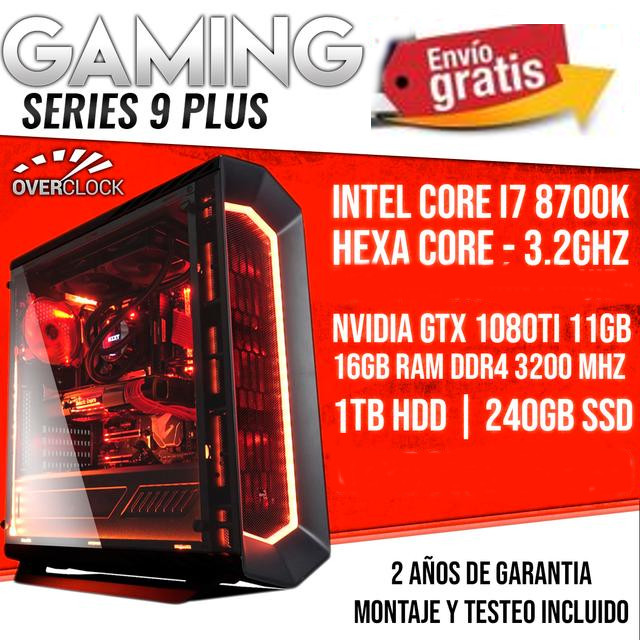
\includegraphics[height=6cm, width=4cm]{pc.jpg} 

\end{tabular}
& \begin{tabular}{l}
\parbox{0.5\linewidth}{
        \textbf{Procesador}: más rápido, mas cores \\
        \textbf{Memoria}: más memoria \\
        \textbf{Disco}: más disco 
}
\end{tabular} \\
\end{tabular}

\end{frame}



\begin{frame}
\frametitle{Jerarquía de memoria}
        \begin{center}
        \textbf\textit{"Procesador más rápido, mas cores"}
        \end{center}
\begin{itemize}
\item \textbf{IMPORTANTE}: es tiempo de utilizar mayor precisión y terminología
\item \texit{Ejemplo: "Microprocesador con un rendimiento mayor que el anterior"} 
\begin{itemize}
\item (Es más adecuado)
\item Buscamos que realice una mayor cantidad de trabajo en el mismo tiempo o,
\item la misma cantidad de trabajo que antes, pero en un tiempo menor. 
\end{itemize}
\end{itemize}
\end{frame}



\begin{frame}
\frametitle{Jerarquía de Memoria}
        \begin{center}
        \textbf{Resumen}
        \end{center}

\begin{itemize}
\item \textbf{Jerarquía de Memoria}: Organización de la memoria de una computadora que permita obtener el \textbf{rendimiento} de una memoria de gran velocidad al \textbf{costo} (precio) de las memorias mas lentas.
\end{itemize}

\end{frame}



\begin{frame}
 \frametitle{Jerarquía de Memoria}
        \begin{center}
        \textbf{DRAM vs SRAM}
        \end{center}
\begin{itemize}
\item Factores: densidad, costos, consumo, rendimiento.
\end{itemize}
\begin{center}
\begin{figure}
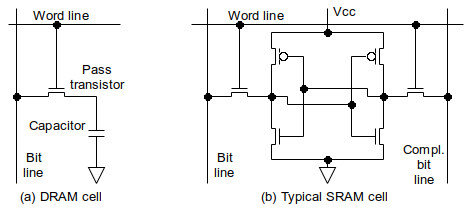
\includegraphics[scale=0.6]{sramvsdram.jpg} 
\caption{DRAM vs SRAM}
\label{DRAM vs SRAM}
\end{figure}
\end{center}
\end{frame}


\begin{frame}
 \frametitle{Jerarquía de Memoria}
        \begin{center}
        \textbf{The Memory Wall}
        \end{center}

Año tras año ...
\begin{itemize}
\item Los microprocesadores nuevos son más rápidos (mejoran el rendimiento). 
\item Las memorias nuevas son más rápidas (mejoran el rendimiento).
\end{itemize}

% \begin{itemize}
% \item Pero, año tras año, el progreso en la tecnología de las CPU es mucho mejor que el de las memorias.
% \end{itemize}

% \begin{itemize}
% \item Desde 1986 hasta el 2005 la velocidad de los microprocesadores aumentaba un 55% cada año, mientras que la memoria mejoraba sólo un 10% la velocidad
% \item Llegará el momento en que la memoria será un muro, en donde el progreso de la tecnología de la CPU no tendrá sentido si no existen mejoras tecnológicas en las memorias.
% \end{itemize}

\begin{center}
\begin{figure}
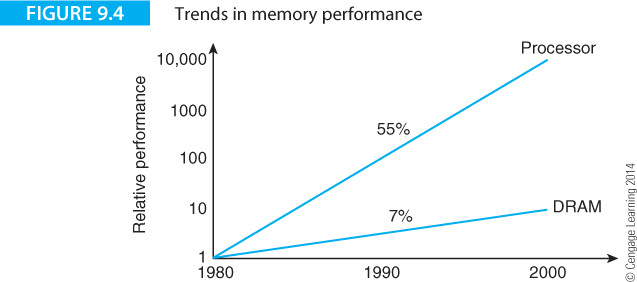
\includegraphics[scale=0.4]{memorywall.jpg} 
\end{figure}
\end{center}
\end{frame}


\begin{frame}
 \frametitle{Jerarquía de Memoria}
        \begin{center}
        \textbf{Jerarquía de Memoria}
        \end{center}
\begin{itemize}
\item Organizar el sistema de memoria dentro de una jerarquía de niveles
\item Objetivo: \textit{obtener el rendimiento de una memoria de gran velocidad al coste de una memoria de baja velocidad, y de tamaño casi ilimitado.}
\end{itemize}
\begin{center}
\begin{figure}
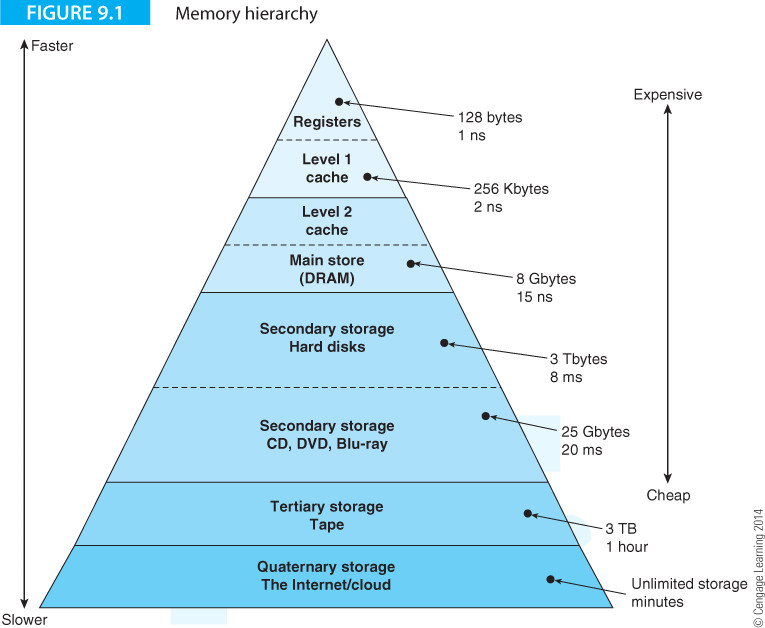
\includegraphics[scale=0.3]{jerarquia.jpg} 
\caption{Jerarquía de Memoria}
\label{Jerarquía de Memoria}
\end{figure}
\end{center}
\end{frame}



\begin{frame}
 \frametitle{Jerarquía de Memoria}
        \begin{center}
        \textbf{Jerarquía de Memoria}
        \end{center}

\begin{tabular}{cl}
\begin{tabular}{c}
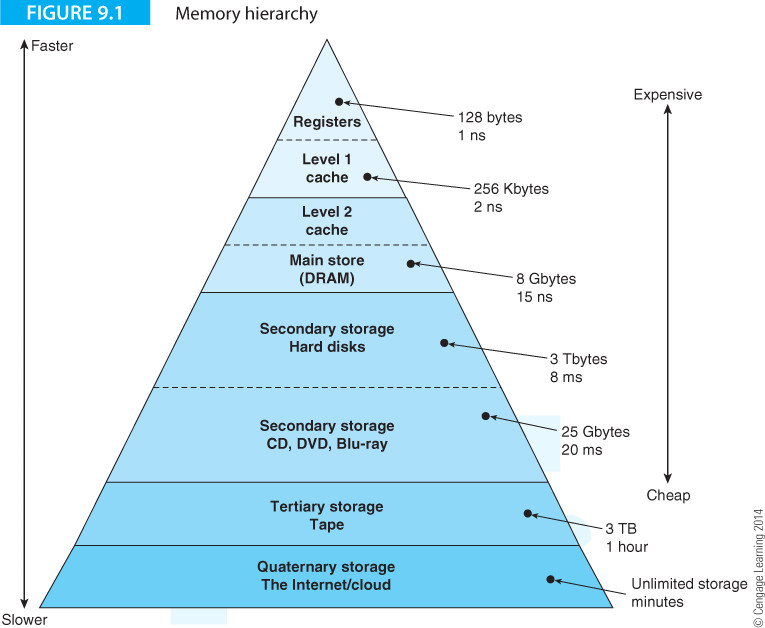
\includegraphics[height=6cm, width=5cm]{jerarquia.jpg} 

\end{tabular}
& \begin{tabular}{l}
\parbox{0.5\linewidth}{
        Organizar el sistema de memoria dentro de una \textbf{jerarquía de niveles}. \\
\\
        \textbf{Objetivo}: \textit{obtener el rendimiento de una memoria de gran velocidad al coste de una memoria de baja velocidad, y de tamaño casi ilimitado.}
}
\end{tabular} \\
\end{tabular}

\end{frame}



\begin{frame}
 \frametitle{Consejos y preguntas}
\begin{center}
\begin{itemize}
\item  ¿Preguntas?
\end{itemize}
\end{center}
\end{frame}


\begin{frame}
 \frametitle{Bibliografía}
        \begin{center}
        \textbf{Material complementario de estudio}
        \end{center}
Apunte de cátedra
\begin{itemize}
\item \textbf{Memoria}, Rafael Ignacio Zurita 2017 (disponible en PEDCO). Versión en español ampliada (con permiso escrito de Prof. Alan Clements y Prof. Hank Levy) de los libros:
\begin{itemize}
\begin{itemize}
\item Computer Organization and Architecture: Themes and Variations, Alan Clements, Cengage Learning, 2013, ISBN: 1285415426, 9781285415420
\item Computer Programming and Architecture the VAX-11, Henry Levy, Digital Press 1980
\end{itemize}
\end{itemize}
\end{itemize}
\end{frame}


\end{document}
